%% Exemplo de utilizacao do estilo de formatacao normas-utf-tex (http://normas-utf-tex.sourceforge.net)
%% Autores: (200?-2011) Hugo Vieira Neto (hvieir@utfpr.edu.br)
%%          (200?-2011) Diogo Rosa Kuiaski (diogo.kuiaski@gmail.com)
%%          (2011-2012) Marcos Talau <talau@users.sourceforge.net>
%% Colaborador:
%%          (2011) César M. Vargas Benitez <cesarvargasb@gmail.com>
%%          (2015) Glauber Gomes de Oliveira Brante <gbrante@utfpr.edu.br>

\documentclass[openright]{Normas/normas-utf-tex} %openright = o capitulo comeca sempre em paginas impares
%\documentclass[oneside]{normas-utf-tex} %oneside = para documentos com numero de paginas menor que 100 (apenas frente da folha)

% force A4 paper format
\special{papersize=210mm,297mm}
\usepackage[hidelinks,plainpages=true, bookmarks=true, breaklinks, pdfstartview=FitH,pdftitle={Nome da Teste},pdfauthor={Nome do autor},pdfsubject={Assunto do documento},pdfkeywords={Palavras-chave}]{hyperref}
\usepackage[hyphenbreaks]{breakurl}
\urlstyle{same}
%configuracao correta das referencias bibliograficas.
\usepackage[alf,abnt-emphasize=bf,bibjustif,recuo=0cm,abnt-etal-cite=2,abnt-etal-list=0,abnt-thesis-year=both]{Normas/abntcite}
\usepackage[brazil]{babel} % pacote portugues brasileiro
\usepackage[utf8]{inputenc} % pacote para acentuacao direta

\usepackage{amsmath,amsfonts,amssymb} % pacote matematico
\usepackage{graphicx} % pacote grafico
%\usepackage{times} % fonte times (substituida pelos dois comandos abaixo - padrao LATEX)
\usepackage[T1]{fontenc}
\usepackage{lmodern}
\usepackage[final]{pdfpages} % adicao da ata
\usepackage{float}
\usepackage{pifont}
\newcommand{\cmark}{\ding{51}}%
\newcommand{\xmark}{\ding{55}}%


% ---------- Preambulo ----------
\instituicao{Universidade Tecnológica Federal do Paraná} % nome da instituicao
\programa{Programa de Pós-Graduação em Sistemas de Energia} % nome do programa
\area{Automação e Sistemas de Energia} % area de concentracao

\documento{Dissertação} % [Dissertacao] ou [Tese]
\documentoingles{Thesis}
\nivel{Mestrado} % [Mestrado] ou [Doutorado]
\curso{Sistemas de Energia}
\titulacao{Mestre} % [Mestre] ou [Doutor]
\autorizacao{(\cmark) Não autorizo a disponibilização de endereço de correio eletrônico para contato.\\
(\xmark) Autorizo a disponibilização do correio eletrônico para contato.} % Autorização de Divulgação de e-mail para contato. Utilize \cmark na linha que preferir e \xmark na linha que não refletir seu desejo
%opções de licença Creative Commons. Marque com X somente a que escolher
\licencaCCBY{} %https://creativecommons.org/licenses/by/4.0/deed.pt
\licencaCCBYNC{X} %https://creativecommons.org/licenses/by-nc/4.0/deed.pt
\licencaCCBYNCND{} %https://creativecommons.org/licenses/by-nc-nd/4.0/deed.pt
\licencaCCBYNCSA{} %https://creativecommons.org/licenses/by-nc-sa/4.0/deed.pt
\licencaCCBYND{} %https://creativecommons.org/licenses/by-nd/4.0/deed.pt
\licencaCCBYSA{} %https://creativecommons.org/licenses/by-sa/4.0/deed.pt

\titulo{Estimativa de localização de alvos em ambientes internos por meio de fusão de algoritmos de Multilateração e Ângulo de Chegada. } % titulo do trabalho em portugues
\title{Indoor target location estimation via Multilateration and Angle of Arrival fusion algorithms.} % titulo do trabalho em ingles

\autor{Andrey Fabris} % autor do trabalho
\cita{FABRIS, Andrey} % sobrenome (maiusculas), nome do autor do trabalho

\palavraschave{Ângulo de Chegada, Bluetooth, Filtros Estocásticos, Multilateração, RSSI. } % palavras-chave do trabalho
\keywords{Angle of Arrival, Bluetooth, Multilateration, RSSI, Stochastic Filters.} % palavras-chave do trabalho em ingles

\comentario{\UTFPRdocumentodata\ apresentada como requisito parcial para obtenção do título de ``\UTFPRtitulacaodata\ em Engenharia Elétrica'' do \UTFPRprogramadata\ da \ABNTinstituicaodata.}

\orientador{Ohara Kerusauskas Rayel} % nome do orientador do trabalho
%\orientador[Orientadora:]{Nome da Orientadora} % <- no caso de orientadora, usar esta sintaxe
\coorientador{João Luiz Rebelatto} % nome do coorientador do trabalho, caso exista
%\coorientador[Coorientadora:]{Nome da Coorientadora} % <- no caso de co-orientadora, usar esta sintaxe

\local{Curitiba} % cidade
\data{2024} % ano


% desativa hifenizacao mantendo o texto justificado.
\tolerance=1
\emergencystretch=\maxdimen
\hyphenpenalty=10000
\hbadness=10000
\sloppy

%---------- Inicio do Documento ----------
\begin{document}
\pdfstringdefDisableCommands{%
	\let\MakeUppercase\relax
}
\capa % geracao automatica da capa
\folhaderosto % geracao automatica da folha de rosto


% insercao da ATA
%\includepdf{ata.pdf}

% dedicatoria
%\begin{dedicatoria}
Texto da dedicatória.
\end{dedicatoria}

% agradecimentos (opcional)
%% agradecimentos
\begin{agradecimentos}
Texto dos agradecimentos.
\end{agradecimentos}

% epigrafe (opcional)
%\begin{epigrafe}
Texto da ep\'igrafe.
\end{epigrafe}

%resumo
\begin{resumo}
Entre as diversas técnicas de radiofrequência utilizadas para obter localização, como o RSSI, Tempo de Voo e Ângulo de Chegada, que são combinadas com algoritmos para determinar o posicionamento de um alvo em ambientes internos, o AdC vem ganhando interesse desde sua incorporação no \textit{Bluetooth Low Energy} 5.1, devido à sua precisão, baixo consumo de energia, custo reduzido e facilidade de implementação. Este trabalho visa reduzir o erro estimado de posição de um alvo por meio de multilateração baseada em RSSI, bem como a posição estimada usando Ângulo de Chegada e RSSI empregando filtros estocásticos, e propor um sistema com precisão aprimorada usando a saída filtrada combinada de ambas as técnicas. Assim, será possível ter um sistema de posicionamento interno BLE 5.1 mais preciso e eficiente em comparação com outras técnicas utilizadas, que pode ser usado para localizar pessoas e ativos em ambientes internos com baixo erro de estimativa. Para alcançar esse objetivo, este trabalho utilizará um banco de dados de medições reais de RSSI e Ângulo de Chegada de um nó alvo BLE 5.1 e um conjunto de antenas em um ambiente de 14x8m, fornecido pela comunidade acadêmica, e aplicará filtros estocásticos aos algoritmos de localização do Ângulo de Chegada e RSSI para reduzir o erro de estimativa. Os erros serão calculados usando o RMSE, e os resultados serão comparados com os da literatura. Espera-se alcançar alta precisão na estimativa da localização de um alvo usando RSSI e Ângulo de Chegada e o sistema combinado proposto alcançará um erro de localização menor do que sistemas separados. A técnica de localização interna apresentada neste trabalho pode ser usada para substituir sistemas de localização de alto custo ou baixa precisão em várias aplicações em indústrias, saúde, comércio, logística e outras áreas.
\end{resumo}
%abstract
\begin{abstract}
Among the various radiofrequency techniques used for obtaining location, such as RSSI, Time of Flight, and Angle of Arrival, which are combined with algorithms to determine the positioning of a target in indoor environments, AoA has been gaining interest since its incorporation into Bluetooth Low Energy 5.1, due to its precision, low energy consumption, low cost, and ease of implementation. This work aims to reduce the estimated position error of a target through multilateration based on RSSI, as well as the estimated position using AoA and RSSI employing stochastic filters, and to propose a system with improved accuracy by using the combined filtered output of both techniques. Thus, it will be possible to have a more precise and efficient BLE 5.1 indoor positioning system compared to other techniques used, which can be used to locate people and assets in indoor environments with low estimation error. To achieve this goal, this work will use a database of real RSSI and AoA measurements from a BLE 5.1 target node and a set of antennas in a 14x8m environment, provided by the academic community, and apply stochastic filters to the AoA and RSSI localization algorithms to reduce estimation error. Errors will be calculated using the RMSE, and the results will be compared with those in the literature. It is expected to achieve high accuracy in estimating the location of a target using RSSI and AoA and the proposed combined system will achieve a lower location error than separate systems. The indoor localization technique presented in this work can be used to replace high-cost or low-precision positioning system in several applications in industries, healthcare, commerce, logistics, and other areas.
\end{abstract}

% listas (opcionais, mas recomenda-se a partir de 5 elementos)
\listadefiguras % geracao automatica da lista de figuras
\listadetabelas % geracao automatica da lista de tabelas
%\listadequadros % adivinhe :)
\listadesiglas % geracao automatica da lista de siglas
\listadesimbolos % geracao automatica da lista de simbolos

% sumario
\sumario % geracao automatica do sumario

% Pacotes necessários quando não se usa sumário
%\renewcommand{\chaptertitlepagestyle}{plainheader}
%\pagenumbering{arabic}



%---------- Inicio do Texto ----------
% recomenda-se a escrita de cada capitulo em um arquivo texto separado (exemplo: intro.tex, fund.tex, exper.tex, concl.tex, etc.) e a posterior inclusao dos mesmos no mestre do documento utilizando o comando \input{}, da seguinte forma:
%\input{intro.tex}
%\input{fund.tex}
%\input{exper.tex}
%\input{concl.tex}

\newcommand\extraPages{1}
\newcounter{savepage}
\setcounter{savepage}{\value{page}+\extraPages}
\setcounter{page}{\value{savepage}}


%---------- Introdução ----------
\chapter{Introdução}
\label{chap:introducao}

O conceito ``Internet da Coisas'' (\sigla{IoT}{Internet das coisas, do inglês \textit{Internet of Things}}, do inglês \textit{Internet of Things}) emergiu nos anos 2000 e, em poucas décadas, tornou-se um pilar fundamental tanto na indústria quanto no cotidiano das pessoas~\cite{Farahsari2022}. A IoT possibilita que dispositivos físicos se conectem, troquem dados e colaborem, transformando objetos cotidianos em dispositivos inteligentes capazes de realizar tarefas complexas~\cite{Fuqaha2015}. A Figura \ref{fig:crescimento_iot-label} apresenta a projeção do crescimento exponencial de dispositivos IoT, em bilhões, entre 2024 e 2030, com um aumento estimado de 242\% em relação a 2019. Esse crescimento exponencial destaca a importância desse segmento, impulsionando a busca por melhorias em aplicações existentes e o desenvolvimento de novas tecnologias.

\begin{figure}[ht]
    \centering
    \caption{Crescimento de dispositivos inteligentes, em bilhões.}
    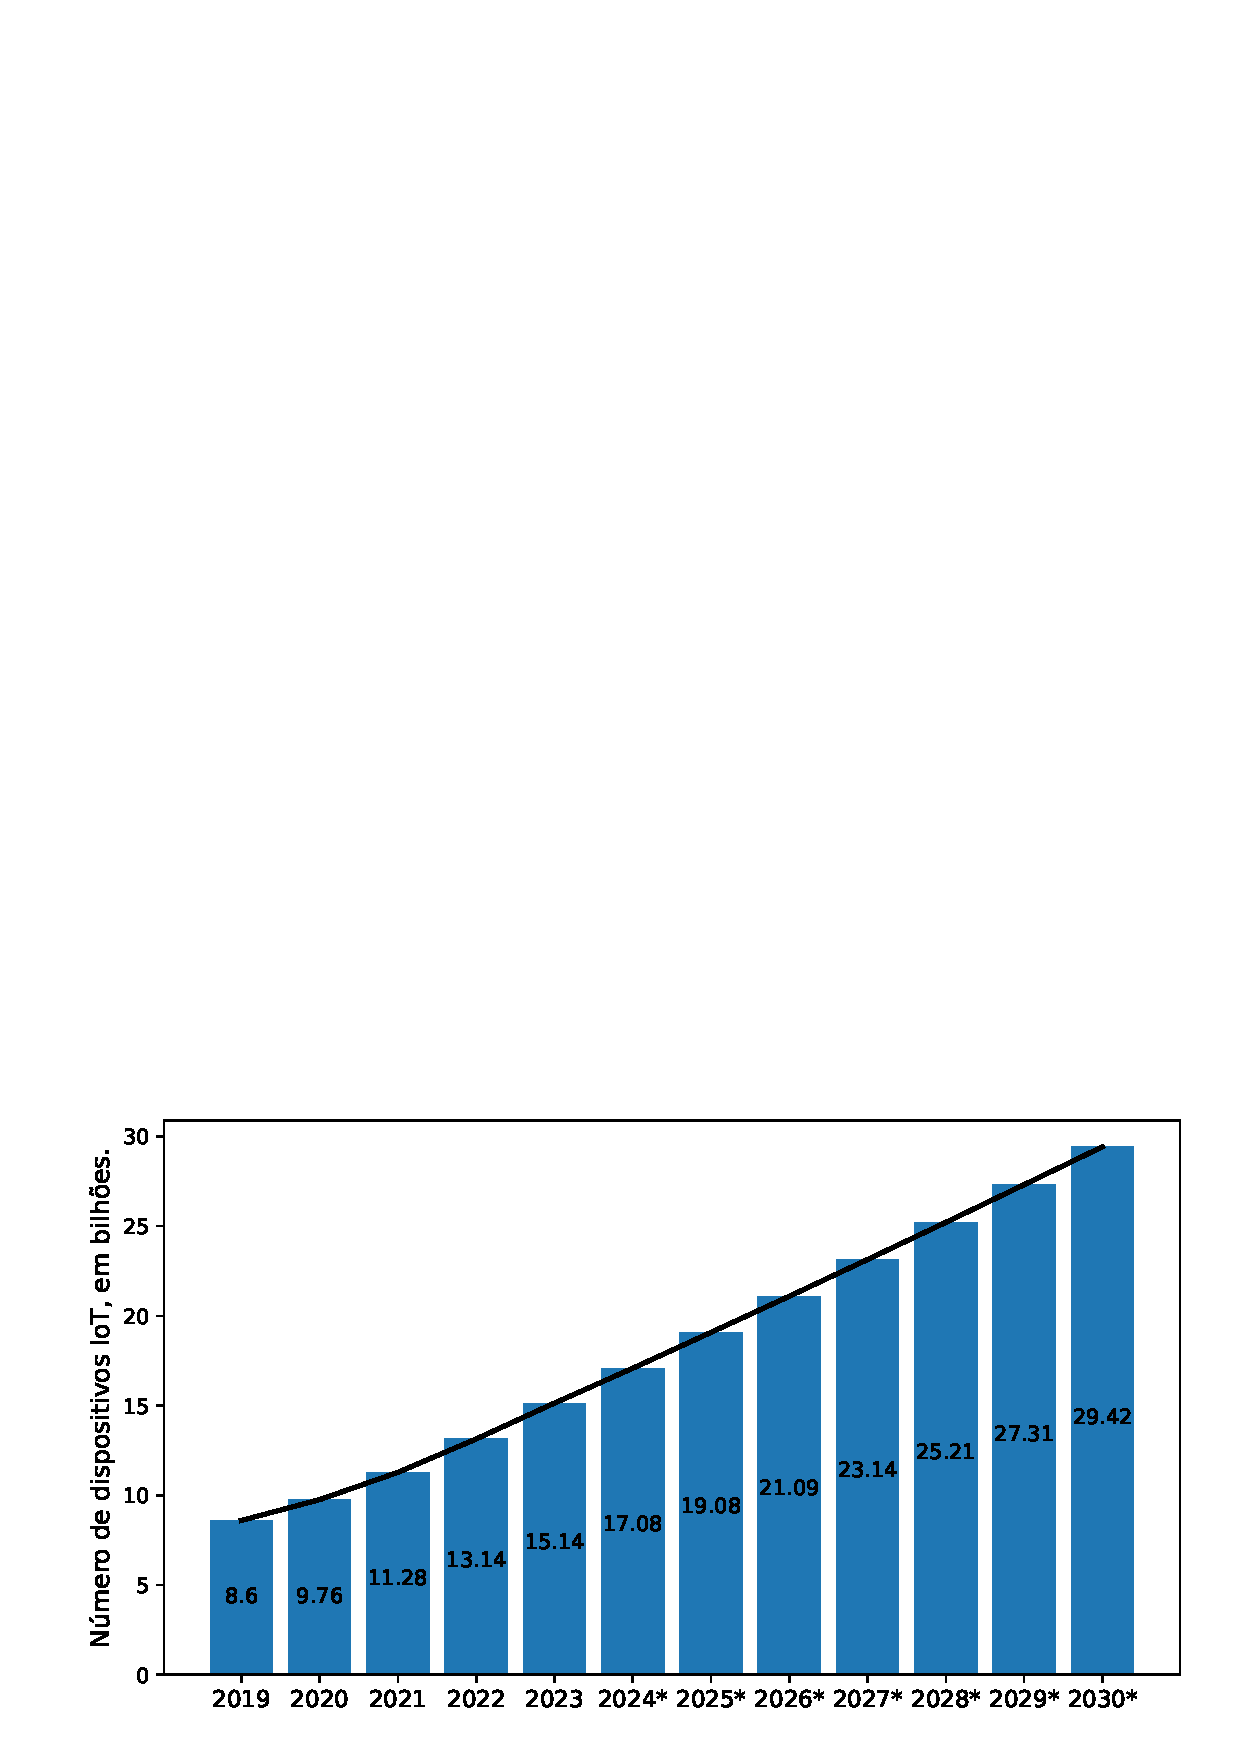
\includegraphics[width=\textwidth]{../Imagens/crescimento_iot.png}
    \fonte{Adaptado de~\cite{Vailshery2023}}
    \label{fig:crescimento_iot-label}
\end{figure}


Dispositivos vestíveis, ou, em inglês, \textit{wearables}, é uma das áreas de dispositivos inteligentes que mais a cada ano, e está se tornando uma parte cada vez mais importante da tecnologia IoT, com seu desenvolvimento evoluindo de acessórios simples para aplicações mais especializadas e práticas~\cite{Dian2020}.A escalabilidade é uma característica fundamental da IoT, permitindo a conexão e gestão de um grande número de dispositivos. Os dispositivos vestíveis contribuem significativamente para essa expansão~\cite{Islam2023}. Através dos sensores e sua conectivade, os dispositivo vestíveis conseguem coletar, enviar dados e tomar decisões, mesmo ao se movimentar junto ao seu usuário. Desta forma, é possível otimizar as aplicações, elevar a qualidade de vida e aumentar a produtividade e segurança de seus usuários. Essa classe inclui dispositivos inteligentes como relógios, braceletes e vestimentas. A Figura \ref{fig:taxonomia_iot-label} demonstra a vasta gama de aplicações para dispositivos inteligentes, com destaque para os dispositivos vestíveis.

\begin{figure}[ht]
    \centering
    \caption{Taxonomia de dispositivos inteligentes.}
    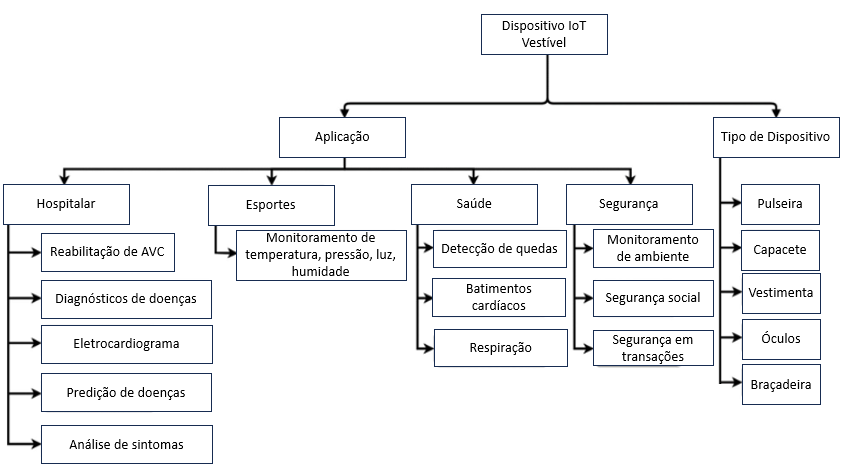
\includegraphics[width=\textwidth]{Imagens/taxonomia_iot.png}
    \fonte{Adaptado de~\cite{Rahmani2022}}
    \label{fig:taxonomia_iot-label}
\end{figure}

 A miniaturização dos componentes eletrônicos e o avanço da tecnologia embarcada possibilitam a integração de múltiplos sensores em dispositivos vestíveis compactos~\cite{Rahmani2022}. A presença de sensores como acelerômetros, giroscópios, \sigla{GPS}{Sistema de Posicionamento Global, do inglês \textit{Global Positioning System}} (do inglês, \textit{Global Positioning System}), medidores de batimentos cardíacos e sensores de temperatura amplia significativamente suas funcionalidades, possibilitando aplicações diversas, desde monitoramento de saúde até rastreamento de atividades físicas.

A preocupação com a qualidade de vida e saúde física, especialmente após a pandemia de COVID-19 em 2020, fez com que os dispositivos vestíveis IoT se tornassem essenciais na vida da maioria das pessoas, graças às medições de batimentos cardíacos, saturação de oxigênio, gasto calórico, distância percorrida, entre outras funções~\cite{Koren2022}. A área biomédica tem usufruido de beneficios como monitoramento à distância de sinais vitais de pacientes, redução de custo e monitoramento em tempo real~\cite{Aledhari2022}. Os \textit{wearables} também podem ser aplicados na segurança dos usuários, por exemplo, para alerta de fadiga durante a condução de um veículo, verificação da qualidade de ar e detecção de quedas, especialmente em idosos \cite{Dian2020}. O emprego da estimativa de localização em tempo real é outra aplicação chave dessa tecnologia, onde a precisão na localização de uma pessoa é benéfica em diversas atividades do dia a dia, como fornecer rotas de navegação para as atividades diárias, e até mesmo ser fundamental para salvar vidas em casos de desastres ambientais ou durante emergências médicas~\cite{Hou2021}. Além de pessoas, é possível acoplar esses equipamentos a outros equipamentos para obter, por exemplo, localizações de robôs móveis~\cite{Tao2021} e de veículos~\cite{Tan2021}.

As aplicações de sistemas de localização podem ser divididas em duas classes: para área externas e internas. Nas áreas externas, a tecnologia principal de posicionamento é o Sistema Global de Navegação por Satélite (\sigla{GNSS}{Sistema Global de Navegação por Satélite, do inglês \textit{Global Navigation Satellite System}}, do inglês \textit{Global Navigation Satellite System}), que pode, por exemplo, rastrear \textit{smartphones} em áreas abertas com uma precisão de nível submétrica~\cite{Liu2022}. Apesar de possuir baixo erro na estimativa de posição em áreas externas, a fraca conectividade entre satélites e dispositivos em ambientes internos os torna ineficazes ou com baixa acurácia~\cite{Guo2020}, sendo necessário o uso de outras tecnologias para esse tipo de ambiente.

Os Sistemas de Posicionamento Interno (\sigla{IPS}{Sistemas de Posicionamento Interno, do inglês \textit{Indoor Positioning System}}, do inglês \textit{Indoor Positioning System}) podem ser utilizados para auxiliar na navegação dentro de estabelecimentos comerciais, localizar pacientes e equipe médica dentro de hospitais, rastrear trabalhadores em minas e construções subterrâneas~\cite{Farahsari2022}.  Diferentes tecnologias de redes \textit{wireless} por radio frequência são utilizadas para estimativa de localização interna, sendo as mais comuns: Wifi, Bluetooth, Identificação por Radio frequência (\sigla{RFID}{Identificação por Radio frequência, do inglês \textit{Radio Frequency Identification}}, do inglês \textit{Radio Frequency Identification}), Banda Ultra Larga (\sigla{UWB}{Banda Ultra Larga, do inglês \textit{Ultra Wide Band}}, do inglês \textit{Ultra Wide Band}), além de Zigbee e LoRaWAN~\cite{Sadowski2018}. Cada uma dessas tecnologias possui seus pontos positivos e negativos, tais como precisão, alcance, custo de processamento, gasto energético e acurácia. A Tabela \ref{tab:ips_comparation} mostra algumas características das tecnologias utilizadas para IPS.

\begin{table}[H]
    \centering
    \caption{Comparação entre tecnologias IPS}
    \begin{tabular}{|c|c|c|c|c|}
        \hline 
         \textbf{Tecnologia} & \textbf{Acurácia} & \textbf{Precisão} & \textbf{Gasto Energético} & \textbf{Custo}  \\
         \hline
         \hline
         Wifi& Métrica & Baixa & Alto & Muito baixo\\
         RFID & Sub-m a Sub-cm& Média a Alta & Baixo a Médio & Baixo-Médio\\
         Bluetooth& Métrica a Sub-m &Baixa&Baixo&Baixo\\
         UWB&Sub-cm a Sub-mm&Alta&Baixo&Médio-Alto\\
         Zigbee&Sub-m&Média&Baixo&Baixo\\
         GNSS&Métrica&Média-Alta&Médio&Médio-Alto \\
         Ultrasom&Sub-m a Sub-mm&Baixa&Baixo&Baixo\\
         
         \hline
    \end{tabular}
    \fonte{Adaptado de \citeonline{Chun2020}.}
    \label{tab:ips_comparation}
\end{table}

Além das tecnologias, IPS pode ser visto como a combinação de mais três princípios: (i) equipamento; (ii) métodos; e (iii) algoritmos. A combinação desses três princípios afeta largamente a performance e precisão do sistema de estimativa de localização em ambientes internos. Os equipamentos, ou em inglês, \textit{hardwares}, são todos os dispositivos físicos utilizados no IPS~\cite{Chun2020}. Exemplos de \textit{hardwares} para IPS incluem:
 \begin{itemize}
     \item Pontos de Acesso (\sigla{AP}{Postos de Acesso, do inglês \textit{Access Point}}, do inglês \textit{Access Point}): Dispositivos que emitem sinais de rádio frequência para estabelecer a comunicação com os dispositivos a serem localizados.

     \item \textit{Beacons} e Tags RFID e Bluetotoh: Pequenos dispositivos que transmitem sinais a intervalos regulares.

     \item  Antenas: Componentes que captam os sinais emitidos pelos APs e pelas tags. Um conjunto de antenas é conhecido como âncora.

     \item Controladores: Dispositivos que processam os sinais recebidos pelas antenas e executam algoritmos de localização.
 \end{itemize}

Existe uma ampla variedade de \textit{hardwares} disponíveis, e a escolha do hardware depende de diversos fatores, como marca, tecnologias, protocolos de transmissão e custo. A qualidade dos equipamentos influencia diretamente na qualidade do IPS.

Diferentes métodos podem ser aplicados para realizar a localização de um objeto dentro de um ambiente interno. A lateração, também conhecida como trilateração ou multilateração (\sigla{MLT}{Multilateção}) consiste em determinar a posição de um objeto com base na distância entre este e múltiplos pontos de referência. Ao medir as distâncias a partir de pelo menos três pontos conhecidos, é possível criar um sistema de equações que permite estimar a posição do objeto. Além da lateração, outro método comum é a angulação ou triangulação, que se baseia na medição do ângulo de chegada (\sigla{AoA}{Ângulo de Chegada, do inglês \textit{Angle of Arrival}}, do inglês \textit{Angle of Arrival}) do sinal emitido pelo objeto. Ao medir o AoA em relação a dois ou mais receptores, é possível triangular a posição do objeto. O método de impressão digital (\sigla{FP}{Impressão Digital, do inglês \textit{Fingerprint}}, do inglês \textit{Fingerprint}), por sua vez, utiliza o Indicador de Intensidade do Sinal Recebido (\sigla{RSSI}{Indicador de Intensidade do Sinal Recebido, do inglês \textit{Received Signal Strength Indication}}, do inglês \textit{Received Signal Strength Indication}) das redes de radiofrequência para estimar a localização. Nesse método, cria-se um banco de dados com os valores de RSSI em diversos pontos do ambiente. Ao comparar o RSSI medido em um determinado ponto com os valores armazenados no banco de dados, é possível estimar a posição do objeto~\cite{Farahsari2022}.

Para cada método de IPS, diferentes algoritmos são empregados para realizar os cálculos da estimva de posição. Esses algoritmos podem ser categorizados em três grupos principais~\cite{Farahsari2022}:

\begin{enumerate}
    \item \textbf{Baseados em tempo}: Baseiam-se na medição do tempo de propagação de um sinal entre dois dispositivos, calculando a distância entre eles a partir da multiplicação desse tempo pela velocidade do sinal. Os principais algoritmos nessa categoria são:  Tempo de Voo (\sigla{ToF}{Tempo de Voo, do inglês \textit{Time of Flight}}, do inglês \textit{Time of Flight}), Diferença no Tempo de Chegada (\sigla{TDoF}{Diferença no Tempo de Chegada, do inglês \textit{Time Difference of Arrival}}, do inglês \textit{Time Difference of Arrival}), e Tempo de Ida e Volta (\sigla{RTT}{Tempo de Ida e Volta, do inglês \textit{Round-trip-time}}, do inglês \textit{Round-trip-time}).

    \item \textbf{Intensidade de Sinal}: Essa é a abordagem mais simples e comum para estimativa de localização interna. Baseia-se na obtenção da distância entre dispositivos a partir da potência e intensidade do sinal. Os indicadores mais utilizados para essa finalidade são: RSSI, Informações do Estado do Canal (\sigla{CSI}{Informações do Estado do Canal, do inglês \textit{Channel State Information}}, do inglês \textit{Channel State Information}), e Potência/Qualidade Recebida do Sinal de Referência (\sigla{PSRP}{Potência Recebida do Sinal de Referência, do inglês \textit{Reference Signal-Received Power}}, do inglês \textit{Reference Signal-Received Power} e \sigla{PSRQ}{Qualidade Recebida do Sinal de Referência, do inglês \textit{Reference Signal-Received Quality}}, do inglês \textit{Reference Signal-Received Quality})

    \item \textbf{Baseado em Ângulo}: Este tipo de algoritmo exige o conhecimento do ângulo formado pelos sinais entre o transmissor e o receptor para determinar a localização. Para isso, podem ser utilizados AoA ou Ângulo de Partida (\sigla{AoD}{Ângulo de Partida, do inglês \textit{Angle of Departure}}, do inglês \textit{Angle of Departure}).
\end{enumerate}

A escolha dos princípios para um IPS depende de diversos fatores, como o ambiente de aplicação, a precisão requerida, o orçamento disponível, os protocolos de integração, e outras características específicas de cada projeto. Por exemplo, em um shopping center, é possível utilizar uma rede Wi-Fi e o método FP com base em medições de RSSI para localizar clientes e aprimorar a experiência de compra~\cite{Lopez2019}. Em hospitais, o RSSI de sinais Bluetooth combinado com o método de lateração pode ser utilizado para rastrear equipamentos e profissionais de saúde~\cite{Casareo2018}. Além disso, a tecnologia RFID pode ser empregada em museus para analisar o comportamento dos visitantes e otimizar a experiência do público~\cite{Vena2021}.
 
O uso do Bluetooth em IPS tem ganhado destaque desde a Bluetooth SIG (\textit{Special Interest Group}) introduziu a especificação Bluetooth 5.1 em 2019. Essa versão aprimorou o Bluetooth \textit{Low Energy} (\sigla{BLE}{\textit{Bluetooth Low Energy}}) ao incluir a tecnologia de determinação de direção (\sigla{DF}{Determinação de Direção, do inglês \textit{Direction Finding}}, do inglês \textit{Direction Finding})~\cite{bluetooth51Core},  possibilitando a triangulação da posição de tags BLE, com precisão de até um metro. Essa triangulação é realizada a partir da diferença de fase do sinal capturada por duas ou mais antenas, permitindo a estimativa da localização com base nos AoD e AoA do sinal, com alta precisão e baixo consumo de energia~\cite{pau_bluetooth_2021}.

Ao posicionar estrategicamente receptores BLE em todo o ambiente interno e equipar os objetos com beacons ou tags BLE, é possível monitorar a localização dos itens desejados de forma precisa e em tempo real. Esses dispositivos BLE podem se comunicar entre si, estabelecendo uma rede de rastreamento contínua e energeticamente eficiente, eliminando a necessidade de frequentes trocas de bateria.

Apesar de ser uma excelente alternativa para a implementação de IPS, a tecnologia BLE está sujeita a desafios inerentes à propagação de sinais em ambientes internos. A transmissão de sinais BLE pode ser atenuada, dispersada ou refletida por obstáculos como paredes, pisos e objetos, além de ser afetada por fatores dinâmicos como a abertura e fechamento de portas, a movimentação de pessoas e as mudanças na disposição dos móveis. Essas interferências geram ruídos e erros nas medições, comprometendo a precisão dos sistemas de localização~\cite{Engström2020}.

Considerando a necessidade de mitigar as incertezas inerentes aos sistemas de posicionamento interno, este trabalho tem como objetivo principal desenvolver e avaliar um IPS robusto, utilizando a tecnologia BLE. A proposta consiste em combinar técnicas de localização, filtragem estocástica e fusão de sensores para reduzir a taxa de erro na estimativa de posição em ambientes internos em relação aos algoritmos e métodos tradicionais.

\section{Introdução ao Problema}\label{sec:intro_problema}

Os IPS baseados em RSSI e AoA são suscetíveis a diversos desafios que comprometem sua precisão. Interferências de sinal, sombreamento e efeitos multicaminhos são fatores que degradam a qualidade dos sinais, enquanto a heterogeneidade dos dispositivos e a variabilidade nas leituras de RSSI e AoA introduzem incertezas nas estimativas de posição~\cite{Guo2023}. Além disso, o equilíbrio entre precisão e consumo de energia é um desafio comum em aplicações de IoT e IPS. Aumentar a frequência e a intensidade das medições para melhorar a precisão resulta em um maior consumo de energia, o que pode limitar a vida útil dos dispositivos e a satisfação do usuário~\cite{Farahsari2022}.

Para garantir a autonomia de dispositivos com IPS integrados, é fundamental priorizar soluções com baixo consumo de energia. Tecnologias como BLE e UWB são promissoras nesse sentido. Além da escolha da tecnologia, o emprego de algoritmos de localização leves e a otimização dos parâmetros de transmissão, como tempo e potência, podem contribuir para reduzir o consumo energético. No entanto, é crucial encontrar um equilíbrio entre o consumo de energia e a precisão do sistema, uma vez que a redução excessiva do consumo pode comprometer a qualidade da localização~\cite{Yao2020, Liu2024, Farahsari2022}.

Os IPS são significativamente afetados por obstáculos presentes nos ambientes, que causam interferências e distorções nos sinais de rádio.  Fenômenos como a não linha de visada (\sigla{NLoS}{não linha de visada, do inglês Non Line of Sight}, do inglês Non Line of Sight), o sombreamento e a propagação multicaminhos resultam em variações significativas na intensidade e na fase dos sinais recebidos, dificultando a estimativa precisa da distância e do ângulo entre transmissores e receptores. Essa incerteza na medição dos sinais compromete a precisão dos sistemas de localização, especialmente em ambientes complexos~\cite{Hayward2022}.

A mobilidade dos dispositivos e de objetos no ambiente introduz uma incerteza intrínseca nas redes de radio frequência sem fio. As constantes mudanças nas condições de propagação, causadas por reflexões, difrações e atenuação, resultam em variações aleatórias nas características do sinal ao longo do tempo. Essa variabilidade torna difícil prever o comportamento do sinal recebido e compromete a qualidade da comunicação, exigindo o desenvolvimento de técnicas robustas para lidar com as incertezas~\cite{Goldsmith2005}.

Conforme \citeonline{Goldsmith2005}, a potência de um sinal transmitido sofre atenuação ao se propagar pelo ambiente, sendo influenciada por dois principais fenômenos: perda de caminho e sombreamento. A perda de caminho é decorrente da dispersão da energia eletromagnética à medida que o sinal se propaga, enquanto o sombreamento é causado pela presença de obstáculos que bloqueiam parcial ou totalmente o sinal, através de processos como absorção, reflexão, dispersão e difração. Quando a atenuação devido ao sombreamento é significativa, o sinal pode ser completamente bloqueado, comprometendo a comunicação.

Para mitigar os efeitos de multicaminhos, sombreamento e outras fontes de ruído que comprometem a precisão das estimativas de posição em sistemas de localização, uma abordagem comum consiste na aplicação de filtragem estocástica. Técnicas como Filtro de Kalman (\sigla{FK}{Filtro de Kalman}), Filtro de Kalman \textit{Unscented} (\sigla{FKU}{Filtro de Kalman \textit{Unscented}}) e Filtro de Partículas (\sigla{FdP}{Filtro de Partículas}) são amplamente utilizados para estimar o estado de um sistema a partir de medidas ruidosas, permitindo reduzir a incerteza nas estimativas de posição~\cite{Ullah2020}.

Proposto por Rudolf Kalman, o FK é uma técnica de filtragem estocástica amplamente empregada para estimar o estado de sistemas dinâmicos lineares a partir de medidas ruidosas. Sua eficiência computacional é atribuída à suposição de que tanto o ruído nas medidas quanto as incertezas na dinâmica do sistema seguem distribuições gaussianas. Essa simplificação permite a obtenção de uma solução analítica recursiva, tornando o FK uma ferramenta poderosa e versátil em diversas áreas de aplicação~\cite{Kalman1960}.

Dada a natureza não linear da maioria dos sistemas reais, o FK, originalmente projetado para sistemas lineares, apresenta limitações. Para lidar com essa complexidade, foram desenvolvidas diversas extensões do FK, como o FKU. A utilização de algoritmos de AoA e AoD, que envolvem funções trigonométricas, introduz não linearidades no processo de estimação de posição. Nesse contexto, os filtros não lineares surgem como uma alternativa eficaz para melhorar a precisão das estimativas. Além disso, a fusão de dados provenientes de múltiplos sensores ou técnicas permite explorar a complementaridade das informações obtidas por cada sensor, resultando em estimativas mais robustas e precisas~\cite{Assa2015}.

A combinação de filtragem estocástica e fusão de sensores em sistemas de posicionamento baseados em BLE representa uma abordagem promissora para alcançar níveis de precisão superiores aos métodos tradicionais. Assim, é possível reduzir as incertezas de medições e melhorar a robustez das estimativas de posição, mesmo em ambientes desafiadores.

\section{Motivação}
\label{sec:motivacao}

A crescente demanda por IPS, tanto no setor comercial quanto no militar, tem impulsionado o desenvolvimento acelerado de tecnologias e sistemas capazes de fornecer soluções precisas em ambientes internos. Essa demanda crescente tem gerado uma vasta gama de aplicações em diversos setores, como saúde, indústria, comércio e logística. A busca por soluções de posicionamento em ambientes internos de baixo custo e alta precisão é fundamental para o sucesso da IoT, impulsionando a inovação nesse campo~\cite{Guo2020, Farahsari2022, Feng2020}.

A configuração dispositivos BLE permite um equilíbrio entre alcance e consumo de energia, tornando essa tecnologia ainda mais atrativa. A facilidade de implantação, o baixo custo, o baixo consumo de energia e a ampla compatibilidade com diversos dispositivos tornaram o BLE uma alternativa competitiva a outras tecnologias de radiofrequência para aplicações de localização em ambientes internos~\cite{Philips2023, Gouzouasis2012}.

A inclusão das características de DF na versão 5.1 do BLE possibilitou alcançar uma precisão submétrica em IPS, e oferece uma oportunidade para superar as limitações de outras tecnologias utilizadas para aplicações de localização interna. Ao combinar essa tecnologia com métodos de estimação de localização e técnicas de filtragem estocástica, é possível desenvolver soluções robustas e precisas para a localização em ambientes internos, otimizando a performance e superando desafios como efeitos de multicaminhos e interferências.

As aplicações de um IPS são vastas e abrangentes. Alguns exemplos de cenários onde o IPS pode ser utilizado incluem: (i) o rastreamento de ativos em ambientes corporativos; (ii) a localização de pessoas em edifícios e comércios; e (iii) a análise do comportamento de clientes em shoppings. 

\section{Procedimentos Medotológicos}
\label{sec:metodologia}

Com auxílio da literatura e da comunidade acadêmica, será utilizado um dataset de medidas reais de RSSI e AoA, obtidas através de dispositivos BLE 5.1, para serem empregados nos algoritmos de IPS. Os dados devem ser coletados em condições estáticas e de movimentação, a fim de comparar a acurácia em diferentes cenários.

Após a estruturação do dataset, será desenvolvido os algoritmos de localização por RSSI e AoA, conforme encontrados na literatura. A implementação dos algoritmos será realizada utilizando a linguagem de programação Python. Em conjunto com os modelos de localização, serão empregados FEs com o intuito de aprimorar a precisão desses algoritmos. Por fim, será proposto um sistema de fusão.

A verificação do desempenho dos algoritmos de localização e dos FEs será realizada por meio da análise da Raiz Quadrada do Erro Médio (\sigla{RMSE}{do inglês, \textit{Root Mean Squared Error}}, do inglês, \textit{Root Mean Squared Error}) e do erro médio da distância entre a posição estimada e a posição real. Essa análise de desempenho demonstrará se a proposta deste trabalho foi adequada para tratar o problema.

\section{Objetivos}
\label{sec:objetivos}

\subsection{Objetivo Geral}
\label{subsec:objetivoGeral}
Estudar, implementar e comparar a acurácia entre diferentes algoritmos de estimativa de localização em ambientes internos. Aplicar filtros estocásticos para reduzir a incerteza das estimativas de posicionamento. Propor um sistema de fusão que supere a acurácia dos métodos isolados.

\subsection{Objetivos Específicos}
\label{subsec:objetivosEspecificos}
\begin{itemize}
    \item  Coletar informações do estado da arte sobre técnicas de localização a partir do BLE 5.1, assim como filtragem estocástica e fusão de sensores;
    \item Obter na literatura medidas reais de RSSI e AoA em ambientes internos similares ao ambiente de estudo;
    \item Definir os algoritmos mais promissores para estimativa, considerando as características do ambiente e os dados disponíveis;
    \item Estabelecer os FEs mais adequados para trabalhar em conjunto com os algoritmos de localização;
    \item Implementar algoritmos e FEs;
    \item Realizar um algoritmo de fusão a partir das técnicas anteriores;
    \item Analisar os resultados através de comparativos de desempenho.
\end{itemize}


\section{Justificativa}
\label{sec:justificativa}

Muitos dos sistemas de IoT existentes ainda dependem de soluções de localização provenientes de tecnologias de localização já estabelecidas, como GNSS e Wi-Fi~\cite{Li2021}. Ou seja, nos últimos anos, os dispositivos BLE têm se destacado como uma alternativa promissora para IPS, graças à sua alta disponibilidade, baixo custo, baixo consumo de energia e facilidade de implantação~\cite{Mackey2020}.

Ao contrário dos ambientes externos, os ambientes internos apresentam uma complexidade muito maior, com formas e tamanhos variados, além da presença ou ausência de objetos fixos e móveis, o que altera significativamente tanto a propagação de sinal de rádio em linha de visada (\sigla{LoS}{do inglês \textit{Line of Sight}}, do inglês \textit{Line of Sight}) quanto NLoS, causando atenuação, dispersão, sombreamento e pontos cegos imprevisíveis, degradando significativamente a precisão do posicionamento interno~\cite{Nessa2020}.

Nesse contexto, a pesquisa e o desenvolvimento de soluções IPS utilizando BLE surgem como alternativa às soluções de localização já estabelecidas, aliando precisão, baixo consumo de energia e fácil integração aos dispositivos IoT. Com a aplicação de FEs, é possível aprimorar significativamente a acurácia dos algoritmos de localização


\section{Cronograma}
\label{sec:cronograma}

O cronograma das etapas desse trabalho encontram-se na Figura \ref{fig:crongrama}.

\begin{figure}[ht]
    \centering
    \caption{Cronograma}
    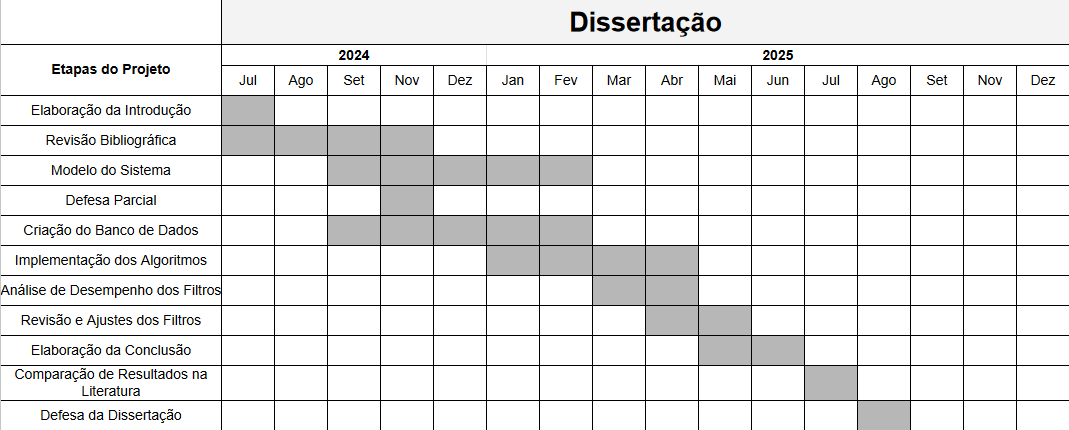
\includegraphics[width=\linewidth]{Imagens/cronograma_dissertacao.png}
    \fonte{Autoria Própria.}
    \label{fig:crongrama}
\end{figure}

\section{Estrutura do Trabalho}
\label{sec:estrutura}

Esse trabalho conterá cinco capítulos, com ordem e conteúdos determinados nesta seção. Este capítulo introdutório compõe-se da apresentação do tema e a introdução ao problema, da motivação da pesquisa, dos objetivos gerais e específicos, e das justificativas para a realização deste trabalho. A introdução também contém as metodologias aplicadas e o cronograma para a sequência da dissertação.

A fundamentação teórica e referência bibliográficas irão compor o segundo capítulo. Nele serão abordados os conceitos e modelos matemáticos para a localização em ambientes internos, e detalhando os conceitos de posicionamento por Bluetooth utilizados neste trabalho. Também será apresentado os FEs empregados, buscando o que melhor se adapta para a modelagem matemática utilizada.

O modelo do sistema, com os algoritmos e solução proposta irão contemplar o terceiro capítulo. O quarto capítulo irá retratar sobre os resultados obtidos e a discussão com resultados encontrados na literatura. O último capitulo desse trabalho abrange a conclusão desse trabalho, a fim de discutir se todos os objetivos propostos foram alcançandos. Por fim, encontram-se as referências utilizadas nesta dissertação.


%---------- Revisão Bibliográfica ----------
\chapter{Revisão da Literatura}
\label{chap:desenv}

Os sistemas de posicionamento baseados em Bluetooth permitem o uso de diversos métodos e algoritmos, cada um com diferentes níveis de precisão, tornando-os amplamente aplicáveis a diferentes cenários, desde rastreamento humano até navegação de robôs. Dessa forma, está se tornando um foco de pesquisa cada vez mais popular para IPS~\cite{Zhuang2022}. Essa crescente popularidade impulsiona a demanda por serviços inteligentes de IoT em ambientes internos. De acordo com um relatório da ResearchAndMarket, o mercado global de IPS foi avaliado em 6,92 bilhões de dólares em 2020 e projeta-se que alcance 23,6 bilhões de dólares até 2025~\cite{Farahsari2022}.

A presença quase universal de transceptores Bluetooth em dispositivos inteligentes contribui significativamente para a escalabilidade dos IPS, reduzindo custos e facilitando a implantação e manutenção. Essas características diferenciam os IPS baseados em Bluetooth de outras tecnologias de localização~\cite{Zhuang2022, Yu2021}, tornando-os uma solução atrativa para diversos setores. Atualmente, as tecnologias de localização Bluetooth têm sido amplamente utilizadas em vários campos, como saúde, varejo, logística e segurança.~\cite{Philips2023}. 

Geralmente, para localização baseada em Bluetooth, assim como em outras tecnologias de localização sem fio, podem ser utilizadas diferentes algoritmos como ToF, TDoA, AoA, AoD e RSSI. Métodos baseados em ToA, TDoA e AoA são mais precisos que os métodos baseados em RSSI. No entanto, eles requerem componentes de alta precisão ou antenas especiais, tornando o sistema caro e complexo para diversas aplicações. Por outro lado, métodos baseados em RSSI possuem a vantagem de baixa complexidade, hardware mais barato e métodos simples~\cite{Assayag2023}. Ao combinar esses algoritmos com técnicas como MLT, FP e triangulação, é possível obter a posição de um alvo.

As ondas de rádio são refletidas, refratadas ou dispersas frequentemente devido à obstrução por obstáculos, o que altera o caminho de propagação do sinal para o receptor, formando uma propagação NLoS e efeitos de multicaminho. A propagação NLoS e os efeitos de multicaminho resultam em perda de acurácia nos resultados de posicionamento~\cite{Yao2020}. Para mitigar esses efeitos, uma abordagem comum consiste na aplicação de técnicas de filtragem estocástica.

Além da aplicação de filtros para melhorar as medidas, a fusão de sensores emerge como outra técnica poderosa. A fusão de sensores coleta informações do ambiente através de múltiplos sensores ou técnicas e, em seguida, funde seus dados para melhorar a qualidade geral da medida~\cite{Assa2015}.

Nas próximas seções, as técnicas de posicionamento, filtragem estocástica e fusão sensorial serão abordadas com maior detalhamento.

\section{Algoritmos para posicionamento}
\label{sec:algoritmos}

\subsection{Geolocalização}
\label{subsec:geolocalizacao}

\subsection{Localização por tempo}
\label{subsec:angulos}

\subsection{Localização por ângulos}
\label{subsec:angulos}

\subsubsection{Equações de ângulos}

\subsection{Localização por intesidade de sinal}
\label{subsec:radiofrequencia}

\subsubsection{Equações de RSSI}

\subsubsection{Equações Hibrido AoA+RSSI}


\section{Filtragem Estocástica}
\label{sec:filtragem}

\subsection{Filtro de Kalman}
\label{subsec:kf}

\subsection{Filtro de Kalman \textit{Unscented}}
\label{subsec:ukf}

\section{Fusão de Sensores}
\label{sec:fusao}



%---------- Modelo do Sistema ----------
\chapter{Modelo do Sistema}
\label{chap:modelosistema}



%---------- Resultados ----------
\chapter{Resultados}
\label{chap:resultados}


%---------- Conclusão ----------
\chapter{Conclusão}
\label{chap:conclusao}


%---------- Referencias ----------
\clearpage % this is need for add +1 to pageref of bibstart used in 'ficha catalografica'.
\label{bibstart}
\bibliography{reflatex} % geracao automatica das referencias a partir do arquivo reflatex.bib
\bibliographystyle{abntex2-alf}
\label{bibend}


%---------- Apendices (opcionais) ----------
%\apendice
%\chapter{Nome do Apêndice}
%\label{chap:apendice}

%Use o comando {\ttfamily \textbackslash apendice} e depois comandos {\ttfamily \textbackslash chapter\{\}}
%para gerar títulos de apêndices.


% ---------- Anexos (opcionais) ----------
%\anexo
%\chapter{Nome do Anexo}
%\label{chap:anexo}

%Use o comando {\ttfamily \textbackslash anexo} e depois comandos {\ttfamily \textbackslash chapter\{\}}
%para gerar títulos de anexos.


% --------- Ordenacao Afabetica da Lista de siglas --------
%\textbf{* Observa\c{c}\~oes:} a ordenacao alfabetica da lista de siglas ainda nao eh realizada de forma automatica, porem
% eh possivel se de realizar isto manualmente. Duas formas:
%
% ** Primeira forma)
%    A ordenacao eh feita com o auxilio do comando 'sort', disponivel em qualquer
% sistema Linux e UNIX, e tambem em sistemas Windows se instalado o coreutils (http://gnuwin32.sourceforge.net/packages/coreutils.htm)
% comandos para compilar e ordenar, supondo que seu arquivo se chame 'dissertacao.tex':
%
%      $ latex dissertacao
%      $ bibtex dissertacao && latex dissertacao
%      $ latex dissertacao
%      $ sort dissertacao.lsg > dissertacao.lsg.tmp
%      $ mv dissertacao.lsg.tmp dissertacao.lsg
%      $ latex dissertacao
%      $ dvipdf dissertacao.dvi
%
%
% ** Segunda forma)
%\textbf{Sugest\~ao:} crie outro arquivo .tex para siglas e utilize o comando \sigla{sigla}{descri\c{c}\~ao}.
%Para incluir este arquivo no final do arquivo, utilize o comando \input{arquivo.tex}.
%Assim, Todas as siglas serao geradas na ultima pagina. Entao, devera excluir a ultima pagina da versao final do arquivo
% PDF do seu documento.


%-------- Citacoes ---------
% - Utilize o comando \citeonline{...} para citacoes com o seguinte formato: Autor et al. (2011).
% Este tipo de formato eh utilizado no comeco do paragrafo. P.ex.: \citeonline{autor2011}

% - Utilize o comando \cite{...} para citacoeses no meio ou final do paragrafo. P.ex.: \cite{autor2011}



%-------- Titulos com nomes cientificos (titulo, capitulos e secoes) ----------
% Regra para escrita de nomes cientificos:
% Os nomes devem ser escritos em italico,
%a primeira letra do primeiro nome deve ser em maiusculo e o restante em minusculo (inclusive a primeira letra do segundo nome).
% VEJA os exemplos abaixo.
%
% 1) voce nao quer que a secao fique com uppercase (caixa alta) automaticamente:
%\section[nouppercase]{\MakeUppercase{Estudo dos efeitos da radiacao ultravioleta C e TFD em celulas de} {\textit{Saccharomyces boulardii}}
%
% 2) por padrao os cases (maiusculas/minuscula) sao ajustados automaticamente, voce nao precisa usar makeuppercase e afins.
% \section{Introducao} % a introducao sera posta no texto como INTRODUCAO, automaticamente, como a norma indica.


\end{document}